
\documentclass[12pt]{article}

\usepackage[bottom = 15mm]{geometry}
\usepackage[utf8]{inputenc}
\usepackage[T2A]{fontenc}
\usepackage[russian]{babel}
\usepackage{graphicx}
\usepackage{caption}
\usepackage{amssymb, amsmath}


\textwidth = 16 cm
\textheight = 23  cm
\oddsidemargin = 0 pt
\topmargin = -1.5 cm
\parindent = 20 pt
\parskip = 0 pt
\flushbottom



\title{{\bf Задача 3.2.1\\ Сдвиг фаз в цепи переменного тока}}
\author{Лось Денис (группа 611)}
\date{5 сентября 2017}




\begin{document}

\maketitle

\paragraph{Цель работы: } изучить влияние активного сопротивления, индуктивности и ёмкости на сдвиг фаз между током и напряжением в цепи переменного тока.

\paragraph{В работе используются: } генератор звуковой частоты, двухканальный осциллограф, магазин ёмкостей, магазин сопротивлений, катушка индуктивности, резисторы, мост переменного тока.

\section*{Введение}
  Достаточно удобным, хотя не очень точным прибором для измерения фазовых соотношений служит электронный осциллограф. Пусть нужно измерить сдвиг фаз между двумя напряжениями $U_1$ и  $U_2$ . Подадим эти напряжения на горизонтальную и вертикальную развёртки осциллографа. Смещение луча по горизонтали и вертикали определяется соотношениями:
\[
	x = x_0 \cos \omega t \qquad y = y_0 \cos  \left(\omega t + \alpha \right),
\] 
где $\alpha$ --- сдвиг между напряжениями $U_1$ и  $U_2$, а $x_0$ и $y_0$ --- амплитуды напряжений, умноженные на коэффициенты усиления соответствующих каналов осциллографа. Исключив время после нескольких преобразований получим, что
\[
	\left(\frac{x}{x_0}\right)^2 + \left(\frac{y}{y_0}\right)^2 + \frac{2 x y}{x_0 y_0} \cos \alpha = \sin^2 \alpha 
\]
\par   
Полученное выражение определяет эллипс, описываемый электронным лучём на экране осциллографа (рис. 1). Ориентация эллипса зависит как от искомого угла, так и от усиления каналов осциллографа. Для расчёта сдвига фаз можно измерить отрезки $2 y_\text{x=0}$ и $2 y_0$. Если подставить эти значения в уравнение эллипса, можно получить:
\[
  \alpha = \pm \arcsin \left(\frac{y_\text{x=0}}{y_0}\right).
\]
Также измерение сдвига фаз удобно проводить следующим образом:
\begin{enumerate}
	\item 
		Подобрать частоту развёртки, при которой на экране осциллографа укладывается чуть больше половины периода синусоиды
	\item
		Отцентрировать горизонтальную ось
	\item
		Измерить расстояние $x_0 $ (рис. 3) между нулевыми значениями одного из сигналов, что соответствует смещению по фазе на $\pi$
	\item
		Измерить расстояние $x$ между нулевыми значениями двух синусоид и пересчитать в сдвиг по фазе $\psi = \pi \cdot x / x_0 $	
\end{enumerate}
\begin{figure}[h!]
	\centering
	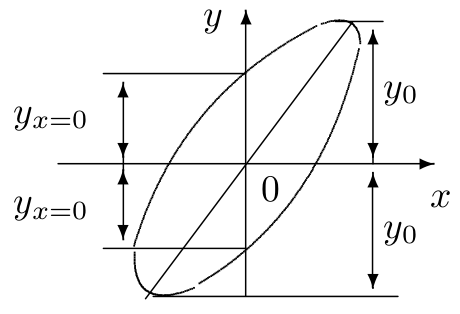
\includegraphics[height=40mm]{image1.png}
	\caption{Эллипс на экране осциллографа}
	\label{image1}
\end{figure}
\par
	На практике часто используются устройства, позволяющие в широких пределах изменять фазу напряжения $\left(0 < \psi < \pi\right)$. Такие устройства называются {\bf фазовращателями}. Схема простого фазовращателя приведена на рис. 2. Она включает в себя два одинаковых резистора 
$R_1$, ёмкость $C$ и переменное сопротивление $R$.
\begin{figure}[h!]
	\centering
	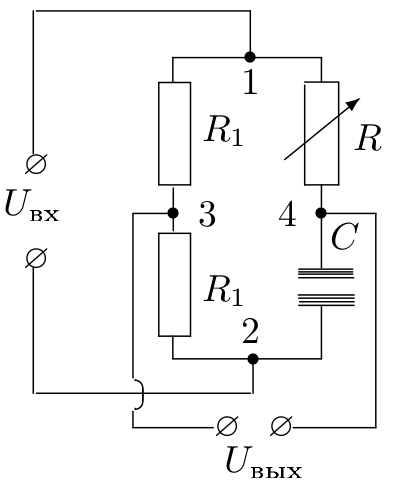
\includegraphics[height=40mm]{image2.png}
	\caption{Принципиальная схема фазовращателя}
	\label{image2}
\end{figure}
\par
	Используя метод комплексных амплитуд, найдём зависимость сдвига фаз между входным напряжением $U_\text{вх} = U_0 \cos \omega t$ и выходным $U_\text{вых}$ от соотношения между импедансами сопротивления $R$ и ёмкости $C$. Для этого выразим выходное напряжение $U_\text{вых}$ через $U_\text{вx}$, параметры контура и частоту внешнего источника $\omega$: $U_\text{34}=f\left(U_\text{12}, R, C, \omega\right)$.
\par
	Обозначим комплексную амплитуду входного напряжения через $\widehat{U_0}$. Тогда напряжение между точками 1 и 3 в силу равенства сопротивлений $R_1$
\[
 	\widehat{U_\text{13}}=\frac{\widehat{U_0}}{2}
\]	
Если фазу напряжения $\widehat{U_\text{вх}}$ положить равной нулю, то $\widehat{U_0}$ будет действительной величиной: $\widehat{U_0}=U_0$. Приняв напряжение в точке 1 равным нулю, получим амплитуду напряжения в точке 3:
\[
	\widehat{U_\text{03}}=\frac{U_0}{2}.
\]
Рассчитаем $\widehat{U_\text{04}}$ --- амплитуду напряжения в точке 4. Импеданс $Z$ последовательно соединённых сопротивления $R$ и ёмкости $C$ равен
\[
	Z = R - \frac{i}{\omega C}
\]	
Для комплексной амплитуды тока $\widehat{I_0}$, проходящего через $R$ и $C$, имеем
\[
	\widehat{I_0}=\frac{U_0}{Z}=\frac{U_0}{R-i/\left(\omega C\right)},
\]	
а для комплексной амплитуды напряжения в точке 4
\[
	\widehat{U_\text{04}}=\widehat{I_0}R=U_0 \frac{R}{R - i/\left(\omega C\right)}
\]	
Выходное напряжение $\widehat{U_\text{вых}}$ равно разности напряжений в точках 3 и 4:
\[
	\widehat{U_\text{вых}}= \widehat{U_\text{04}}-\widehat{U_\text{03}}=\widehat{U_\text{04}} - U_0 / 2 = \frac{U_0}{2} \frac{R + i/\left(\omega C\right)}{R - i/\left(\omega C\right)}.	
\]	
В числитель и знаменатель последнего выражения входят комплексно-сопряжённые величины, модули которых одинаковы, поэтому величина выходного напряжения не меняется при изменении $R$. Модуль $U_\text{вых}$ всегда равен $U_0 / 2$ --- половине $U_\text{вх}$. Сдвиг фаз между входным и выходным напряжениями равен $2 \arctg\left(1 / \left(\omega R C\right)\right)$ и меняется от $\pi$ (при $R \to 0$) до $0$ (при $R \to \infty$).	
\section*{Экспериментальная установка}
\par
	Схема для исследования сдвига фаз между током и напряжением в цепи переменного тока представлена на рис. 3. Эталонная катушка $L$, магазин ёмкостей $C$ и магазин сопротивлений $R$ соединены последовательно и через дополнительное сопротивление $r$ подключены к источнику синусоидального напряжения --- звуковому генератору.
\clearpage	 
\begin{figure}[h!]
	\centering
	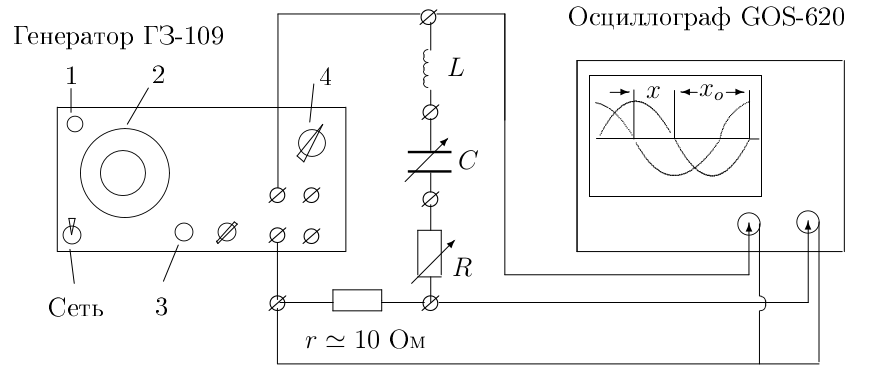
\includegraphics[width=15cm]{image3.png}
	\caption{Схема установки для исследования сдвига фаз между током и напряжением}
	\label{image3}
\end{figure}	
\par
	Сигнал, пропорциональный току, снимается с сопротивления $r$, пропорциональный напряжению --- с генератора. Оба сигнала подаются на универсальный осциллограф. Данный осциллограф имеет два канала вертикального отклонения, что позволяет одновременно наблюдать на экране два сигнала.
\par 	
	Схема фазовращателя, изображённая на рис. 4, содержит два одинаковых резистора $R_1$, смонтированных на отдельной плате, магазин сопротивлений $R$ и магазин ёмкостей $C$.
\begin{figure}[h!]
	\centering
	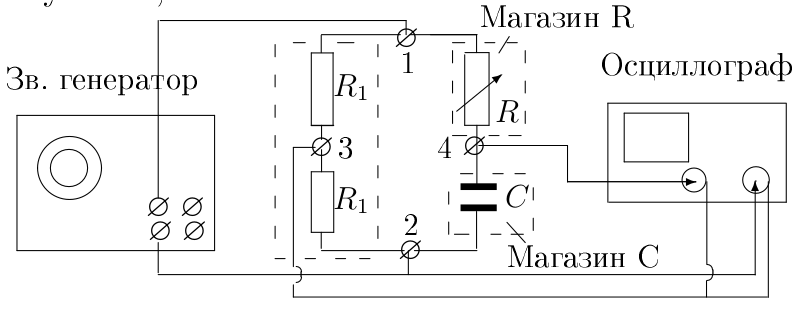
\includegraphics[width=15cm]{image4.png}
	\caption{Схема установки для исследования фазовращателя}
	\label{image4}
\end{figure}
\section*{Ход работы}
\par
	В данной работе предлагается исследовать зависимости сдвига фаз между током и напряжением от в $RC$ и $RL$ цепях; определить добротность колебательного контура, сняв зависимость сдвига фаз от частоты вблизи резонанса; оценить диапазон работы фазовращателя.	
\paragraph{Исследование зависимости сдвига фаз между током и напряжением от $R$ в $RC$ цепи}
\begin{enumerate}
	\item
		В схеме, собранной согласно рис. 3, закоротим катушку, подключив оба провода, идущих к катушке, на одну клемму. Установим $C = 0.5$ мкФ и $v = 1$ кГц. Реактивное сопротивление $X_1 = 1 / \left(\omega C \right) = 1 / \left(2 \pi v C\right) = 318$ Ом. Увеличивая сопротивление $R$ от нуля до $10 \cdot X_1$, проведём измерения сдвига фаз $\psi = \pi \cdot x / x_0$.
		\begin{table}[h!]
			\centering
			\begin{tabular}{|c|c|c|c|}
			\hline
			$R$, Ом  &  $x$, клетки & $x_0$, клетки & $\psi$, рад \\
 			\hline
 			500 & 0.6 & 3.6 & $0.167 \pi$ \\
 			\hline
 			1000 & 0.4 & 3.8 & $0.105 \pi$ \\
 			\hline
 			1500 & 0.2 & 3.6 & $0.056 \pi$ \\
 			\hline
 			2000 & 0.2 & 4.2 & $0.048 \pi$ \\
 			\hline
 			2200 & 0.2 & 4.4 & $0.045 \pi$ \\ 						
			\hline
			2500 & 0.2 & 5.2 & $0.038 \pi$ \\
			\hline
			\end{tabular}
			\label{table1}
		\end{table}		
	\item
		В данной экспериментальной установке $r=12.4$ Ом, что было измерено с помощью моста E7-8. Построим график зависимости $\tg \psi = f(1 / \left(\omega C 	R_s \right))$ (рис.5), где $R_s = R + r$ --- суммарное активное сопротивление цепи.  
		\begin{table}[h!]
 			\centering
 			\begin{tabular}{|c|c|c|}
 			\hline
 			$1 / \left(\omega C R_s \right)$ & $\tg \psi$ & $\Delta_\text{$\tg \psi$}$ \\
 			\hline
 			0.621 & 0.579 & 0.048\\
 			\hline
 			0.314 & 0.342 & 0.043\\
 			\hline
 			0.210 & 0.177 & 0.044\\
 			\hline
 			0.158 & 0.152 & 0.038\\
 			\hline
 			0.144 & 0.142 & 0.036\\ 			
 			\hline
 			0.127 & 0.120 & 0.031\\ 			 			 			
 			\hline
 			\end{tabular}			
			\label{table2}
		\end{table}
\end{enumerate}		
\paragraph{Исследование зависимости сдвига фаз от $R$ в $RL$ цепи}
\begin{enumerate}
	\item
		В схеме, собранной согласно рис.3, закоротим магазин ёмкостей. Установим $L = 500$ мГн, $v = 1$ кГц. Реактивное сопротивление $X_2 = \omega L = 3142$ Ом. Увеличивая сопротивление $R$ от нуля до $10 \cdot X_2$, проведём измерение сдвига фаз.
		\begin{table}[h!]
		\centering
		\begin{tabular}{|c|c|c|c|}
			\hline
			$R$, Ом  &  $x$, клетки & $x_0$, клетки & $\psi$, рад \\
 			\hline
 			500 & 0.8 & 2 & $0.400 \pi$\\
 			\hline
 			2000 & 0.5 & 1.8 & $0.278 \pi$  \\
 			\hline
 			3000 & 0.5 & 2.2 & $0.227 \pi$\\
 			\hline
 		    4000 & 0.3 & 1.8 & $0.167 \pi$\\
 			\hline
 			5000 & 0.3 & 2.2 & $0.136 \pi$\\ 						
			\hline
			6000 & 0.2 & 2 & $0.100 \pi$\\
			\hline
			\end{tabular}
		\label{table3}
		\end{table}		
		\newpage 		
		\begin{figure}[h!]
			\centering
			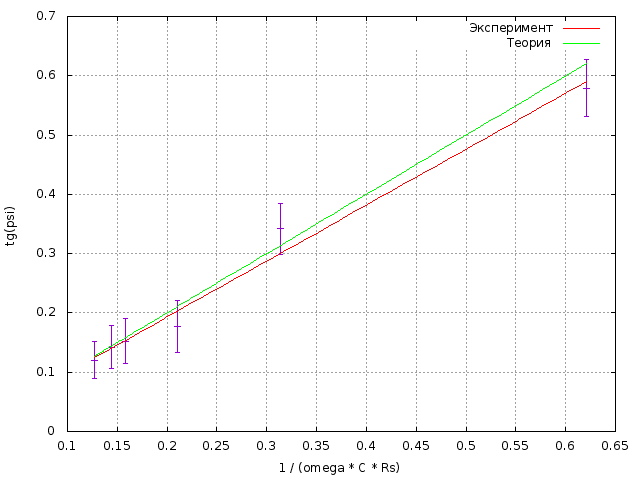
\includegraphics[width = 15cm,height = 8cm]{plot1.png}
			\caption{График зависимости $\tg \psi$ от $ 1 / \left(\omega C R_s \right)$ для $RC$ цепи}
			\label{plot1}
		\end{figure}
	\item	
		В данной экспериментальной установке $R_L = 342.48$ Ом, что было измерено с помощью моста E7-8. Построим график $\tg \psi = f(\omega L / R_s)$, где $R_s = R + r + R_L$.
        \begin{figure}[h!]
			\centering
			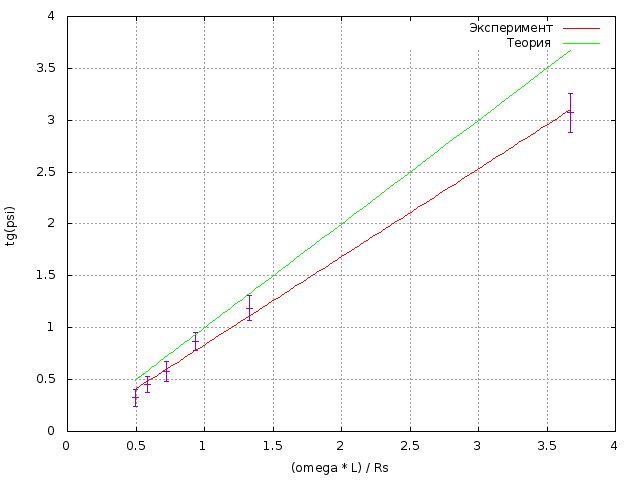
\includegraphics[width = 15cm,height = 8cm]{plot2.png}
			\caption{График зависимости $\tg \psi$ от $ \left(\omega L\right) / R_s $ для $RL$ цепи}
			\label{plot2}
		\end{figure}
		\newpage
		\begin{table}[h!]
			\centering
			\begin{tabular}{|c|c|c|}
			\hline
			$\omega L / R_s$ & $\tg \psi$ & $\Delta_\text{$\tg \psi$}$ \\
			\hline
			3.67 & 3.07   & 0.192  \\
			\hline
			1.33 & 1.19   & 0.120\\
			\hline 
			0.936 & 0.865 & 0.087\\
			\hline
			0.721 & 0.579 & 0.097\\
			\hline
			0.587 & 0.455 & 0.076\\
			\hline
			0.494 & 0.324 & 0.081 \\						
			\hline
			\end{tabular}
			\label{table4}
		\end{table}		
\end{enumerate}
\paragraph{Исследование зависимости сдвига фаз от частоты в $RCL$ цепи}
\begin{enumerate}
	\item
		В цепи, собранной согласной рис.3, установим значение $C = 0.5$ мкФ, $L = 50$ мГн и $R = 0$ Ом. Теоритическая резонансная частота $v_0 = 1/\left(2 \pi \sqrt{LC}\right) = 1006.58$ Гц. Так как $L_\text{реал} = 83.35$ мГн, что было измерено с помощью моста E7-8, то $v_\text{0 реал} = 781$ Гц. 
	\item
		Подберём частоту звукового генератора так, что получить резонанс. При резонансе сдвиг фаз $\psi = 0$ и нулевые значения двух синусоид должны совместиться. Полученная таким образом частота $v_\text{рез} = 760$ Гц. Меняя частоту в обе стороны от резонансного значения,снимем зависимость сдвига фаз от частоты.
		\begin{table}[h!]
			\centering
			\begin{tabular}{|c|c|c|c|}
			\hline
			$v$, Гц  &  $x$, клетки & $x_0$, клетки & $|\psi|$, рад \\
 			\hline
 			1200 & 0.6 & 2 & $0.300 \pi$\\
 			\hline
 			1100 & 0.4 & 1.6 & $0.250 \pi$  \\
 			\hline
 			1000 & 0.4 & 1.9 & $0.211 \pi$\\
 			\hline
 		    900 & 0.4 & 2.2 & $0.182 \pi$\\
 			\hline
 			850 & 0.2 & 2.5 & $0.080 \pi$\\ 						
			\hline
			800 & 0.2 & 2.8 & $0.071 \pi$\\
			\hline
			\hline	
			650 & 0.2 & 2.2 & $0.091 \pi$\\
 			\hline
 			600 & 0.4 & 2.2 & $0.182 \pi$  \\
 			\hline
 			550 & 0.5 & 2.3 & $0.217 \pi$\\
 			\hline
 		    500 & 0.6 & 2.4 & $0.250 \pi$\\
 			\hline
 			450 & 0.8 & 2.6 & $0.308 \pi$\\ 						
			\hline
			\end{tabular}
			\captionsetup{labelformat = empty}
			\caption{Таблица $|\psi| = f(v)$ для $R = 0$ Ом}
			\label{table5}
		\end{table}
	\item
		Установим $R = 100$ Ом и повторим измерения пункта 2.
	\item
		Построим графики $|\psi| = f(v/v_\text{рез})$ для $R = 0$ Ом и $R = 100$ Ом. Определим по графикам добротность контура $Q = v_\text{рез} / \left(2\Delta v\right)$, где $2 \Delta v / v_\text{рез}$ --- ширина графика при сдвиге фаз $\psi = \pi / 4$.
		\newpage		
		\begin{table}[h!]
			\centering
			\begin{tabular}{|c|c|c|c|}
			\hline
			$v$, Гц  &  $x$, клетки & $x_0$, клетки & $|\psi|$, рад \\
			\hline
 			1300 & 1.6 & 5.8 & $0.276 \pi$ \\
 			\hline 			
 			1200 & 1.4 & 5.6 & $0.250 \pi$\\
 			\hline
 			1100 & 1.2 & 5.4 & $0.222 \pi$  \\
 			\hline
 			1000 & 0.8 & 5 & $0.160 \pi$\\
 			\hline
 		    900 & 0.6 & 4.8 & $0.125 \pi$\\ 						
			\hline
			800 & 0.4 & 4.6 & $0.087 \pi$\\
			\hline
			\hline	
			650 & 0.2 & 2.6 & $0.077 \pi$\\
 			\hline
 			600 & 0.4 & 2.7 & $0.148 \pi$  \\
 			\hline
 			550 & 0.9 & 5.4 & $0.167 \pi$\\
 			\hline
 		    500 & 1.2 & 5.4 & $0.222 \pi$\\
 			\hline
 			450 & 1.1 & 4.4 & $0.250 \pi$\\ 
 			\hline
 			400 & 1.3 & 4.4 & $0.295 \pi$\\						
			\hline
			\end{tabular}
			\captionsetup{labelformat = empty}
			\caption{Таблица $|\psi| = f(v)$ для $R = 100$ Ом}
			\label{table6}
		\end{table}
		\begin{figure}[h!]
			\centering
			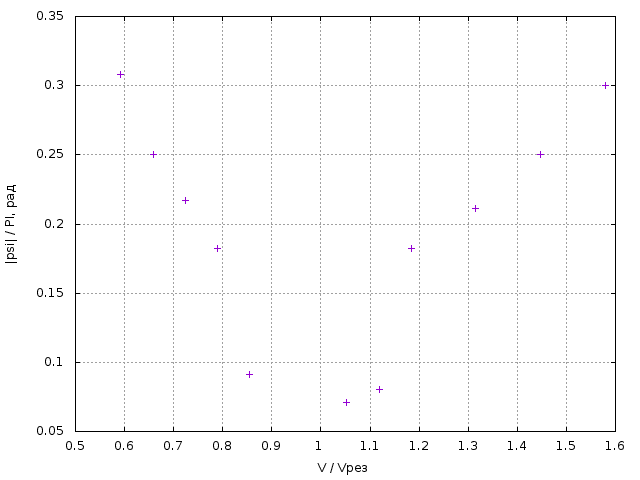
\includegraphics[width = 11cm,height = 5.5cm]{plot3.png}
			\caption{График зависимости $|\psi|$ от $ v/v_\text{рез}$ для $RCL$ цепи при $R = 0$ Ом}
			\label{plot3}
		\end{figure}
		\begin{figure}[h!]
			\centering
			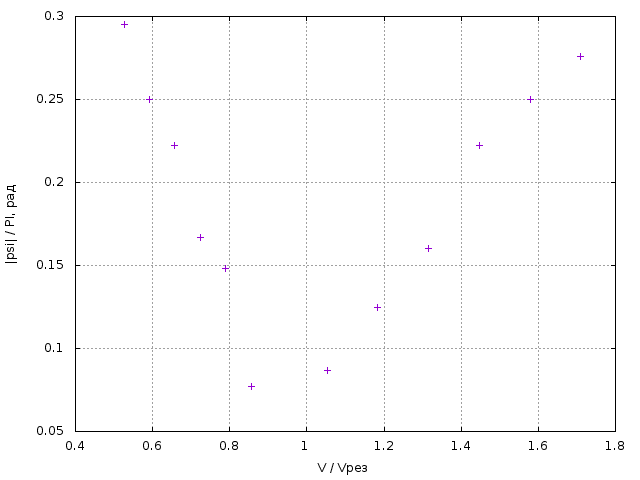
\includegraphics[width = 11cm,height = 5.5cm]{plot4.png}
			\caption{График зависимости $|\psi|$ от $ v/v_\text{рез}$ для $RCL$ цепи при $R = 100$ Ом}
			\label{plot4}
		\end{figure}
	\item 
		Из графиков получаем, что
\begin{align*}
	Q_\text{R = 0} &= 1.27 \\
	Q_\text{R = 100} &= 1.01
\end{align*} 
Тогда как теоритически
\[
	Q = \frac{1}{R} \, \sqrt{\frac{L}{C}}
\]
 а значит, 
\begin{align*}
Q_\text{R = 0 теор} &= 1.14\\
Q_\text{R = 100  теор} &= 0.90
\end{align*}				
\end{enumerate}
\paragraph{Исследование работы фазовращателя}
\begin{enumerate}
	\item
		Соберём схему согласно рис.4. Установим $C = 0.5$ мкФ, $v = 1$ кГц. Можем видеть, что при $R = 0$ Ом будет $|\psi| = 0$, а при приближении $R$ к $10$ кОм, $|\psi|$ приближается к $\pi$. Заметим, что $|\psi|$ равен $\frac{\pi}{2}$ при $318$ Ом, т.е при $1 / \left(\omega C\right))$.
	\item
		Построим векторную диаграмму для фазовращателя. Входное напряжение приложено как к левой части, так и к правой части фазовращателя, т.е $U_\text{вx} = U_\text{R1} + U_\text{R2}$. Напряжение на конденсаторе отстаёт по фазе на $\frac{\pi}{2}$ от напряжения $U_R$, а следовательно, на векторной диаграмме они будут всегда перпендикулярны и будут опираться на диаметр окружности. Выходной вектор --- это вектор между точками 3 и 4 на схеме установки, который будет радиусом этой окружности и будет изменяться только по направлению, но не по модулю. Он будет поворачиваться от $0$ до $-\pi$, если отсчитывать угол от направления вектора входного напряжения.
	\begin{figure}[h!]
		\centering
		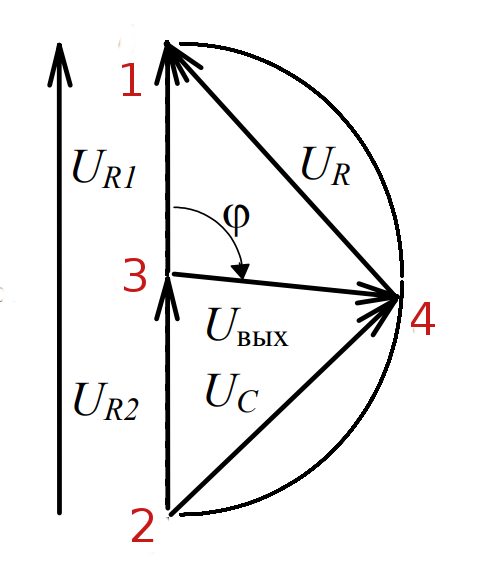
\includegraphics[height = 7cm]{image5.png}
		\caption{Векторная диаграмма для фазовращателя}
	\end{figure}		 	
\end{enumerate}




					
	
\end{document} 

